\documentclass[a4paper,11pt,twoside]{article}
\usepackage[utf8x]{inputenc}
\usepackage{geometry}
\usepackage[T1]{fontenc}
\usepackage[english]{babel}
\usepackage{graphicx}
\usepackage{amsmath}
\usepackage{amssymb}
\usepackage{setspace}
\usepackage{fancyhdr}
\usepackage{wrapfig}
\usepackage{subfig}
\usepackage{hyperref}
\usepackage{sidecap}
\usepackage{theorem}
\usepackage{thc}
\usepackage{url}
\usepackage{booktabs}
\usepackage{multirow}

\def\ttbar{\ensuremath{t\bar{t}}}
\def\ttbaremu{\ensuremath{t\bar{t}~e-\mu}}
\def\pt{\ensuremath{p_{\mathrm{T}}}} % Subscript roman not italic (EE)

%
% +--------------------------------------------------------------------+
% |                                                                    |
% |  Some useful units                                                 |
% |                                                                    |
% +--------------------------------------------------------------------+
%
\def\TeV{\ifmmode {\mathrm{\ Te\kern -0.1em V}}\else
                   \textrm{Te\kern -0.1em V}\fi}%
\def\GeV{\ifmmode {\mathrm{\ Ge\kern -0.1em V}}\else
                   \textrm{Ge\kern -0.1em V}\fi}%
\def\MeV{\ifmmode {\mathrm{\ Me\kern -0.1em V}}\else
                   \textrm{Me\kern -0.1em V}\fi}%
\def\keV{\ifmmode {\mathrm{\ ke\kern -0.1em V}}\else
                   \textrm{ke\kern -0.1em V}\fi}%
\def\eV{\ifmmode  {\mathrm{\ e\kern -0.1em V}}\else
                   \textrm{e\kern -0.1em V}\fi}%
\let\tev=\TeV
\let\gev=\GeV
\let\mev=\MeV
\let\kev=\keV
\let\ev=\eV

\def\TeVc{\ifmmode {\mathrm{\ Te\kern -0.1em V}/c}\else
                   {\textrm{Te\kern -0.1em V}/$c$}\fi}%
\def\GeVc{\ifmmode {\mathrm{\ Ge\kern -0.1em V}/c}\else
                   {\textrm{Ge\kern -0.1em V}/$c$}\fi}%
\def\MeVc{\ifmmode {\mathrm{\ Me\kern -0.1em V}/c}\else
                   {\textrm{Me\kern -0.1em V}/$c$}\fi}%
\def\keVc{\ifmmode {\mathrm{\ ke\kern -0.1em V}/c}\else
                   {\textrm{ke\kern -0.1em V}/$c$}\fi}%
\def\eVc{\ifmmode  {\mathrm{\ e\kern -0.1em V}/c}\else
                   {\textrm{e\kern -0.1em V}/$c$}\fi}%
\let\tevc=\TeVc
\let\gevc=\GeVc
\let\mevc=\MeVc
\let\kevc=\keVc
\let\evc=\eVc

\def\TeVcc{\ifmmode {\mathrm{\ Te\kern -0.1em V}/c^2}\else
                   {\textrm{Te\kern -0.1em V}/$c^2$}\fi}%
\def\GeVcc{\ifmmode {\mathrm{\ Ge\kern -0.1em V}/c^2}\else
                   {\textrm{Ge\kern -0.1em V}/$c^2$}\fi}%
\def\MeVcc{\ifmmode {\mathrm{\ Me\kern -0.1em V}/c^2}\else
                   {\textrm{Me\kern -0.1em V}/$c^2$}\fi}%
\def\keVcc{\ifmmode {\mathrm{\ ke\kern -0.1em V}/c^2}\else
                   {\textrm{ke\kern -0.1em V}/$c^2$}\fi}%
\def\eVcc{\ifmmode  {\mathrm{\ e\kern -0.1em V}/c^2}\else
                   {\textrm{e\kern -0.1em V}/$c^2$}\fi}%
\let\tevcc=\TeVcc
\let\gevcc=\GeVcc
\let\mevcc=\MeVcc
\let\kevcc=\keVcc
\let\evcc=\eVcc

\def\mt{\ensuremath{m_{t}}}

%
% +--------------------------------------------------------------------+
% |                                                                    |
% |  Particles                       |
% |                                                                    |
% +--------------------------------------------------------------------+

\def\Zzero{\ensuremath{Z}}
\def\Zboson{\ensuremath{Z}}
\def\Wplus{\ensuremath{W^+}}
\def\Wminus{\ensuremath{W^-}}
\def\Wboson{\ensuremath{W}}%
\def\Wpm{\ensuremath{W^{\pm}}}%
\def\Wmp{\ensuremath{W^{\mp}}}%


\setlength{\headheight}{15pt}

\geometry{left=3 cm,right=3 cm, top=3.5 cm, bottom=3.5 cm}
\fancyhf{}
\fancyhead[RO,LE]{\footnotesize{\leftmark}}
\fancyhead[LO,RE]{\thepage}

\pagestyle{fancy}

\renewcommand\maketitle{
\begin{titlepage}

 \begin{center}
 
 \begin{figure}[htpb]
\rule{1 \textwidth}{1pt}\\
 \smallskip  
 \end{figure}

\vfill

\textbf{
\begin{huge}
Unfolding technique for the \ttbaremu~analysis \\via machine learning (deep neural network)
\end{huge}
}

\vspace{0.4cm}

\begin{Large}
 \textit{DESY Summer Student Programme, 2019}
\end{Large}

\vspace{1cm}


\begin{tabular}{ccc}
\LARGE{Luiza Adelina Ciucu} \vspace{0.15cm}\\
\large{\textit{University of Geneva, Switzerland}}\\
\end{tabular}
  
\vspace{0.7cm}
\large{Supervisors:\\Thorsten Khul, Yichen Li}\\
\vspace{0.7cm}

\includegraphics[width=0.4\textwidth]{./plots/LogoATLAS.png}\\
\vspace{0.7cm}
\Large{\today}

\end{center}

\vfill

\begin{abstract}
The validity of the Standard Model is tested also through precision measurements of the top quark properties. Inferring from measured quantities what happens in reality in nature is called unfolding. Traditional unfolding methods via migration matrices have limitations. A new method of unfolding using machine learning via neural networks (NN) has been proposed in a paper. In this report this NN technique is applied for unfolding the jet energy transverse momentum in the context of the \ttbaremu~analysis in ATLAS. A deep NN architecture is optimised for this task, leading to an improved performance over the default architecture suggested in the paper.
\end{abstract}

\vfill

  \begin{center}
 \rule{1 \textwidth}{1pt}\\
 \end{center}

% Please choose eg eps or jpg if you work with latex2pdf or not
\begin{figure}[htbp]
     \begin{minipage}{0.5\textwidth}
      \centering
      
\includegraphics[width=0.66\columnwidth]{./plots/LogoUGeneva.jpg}
     \end{minipage}\hfill
     \begin{minipage}{0.5\textwidth}
      \centering
      
\includegraphics[width=0.33\columnwidth]{./plots/LogoDESY.png}
     \end{minipage}
   \end{figure}

\end{titlepage}}

\begin{document}

\maketitle

\tableofcontents
\newpage
\setcounter{page}{1}

\section{Introduction}
\label{sec:Introduction}

\subsection{The Standard Model}
\label{sec:StandardModel}

The Standard Model (SM) is a theory that describes the elementary particle (fermions and bosons) and their interactions via three fundamental forces. The SM elementary particles are illustrated in Figure~\ref{fig:SMParticles} and described in more detail below.

\begin{figure}[h]
  \centering
  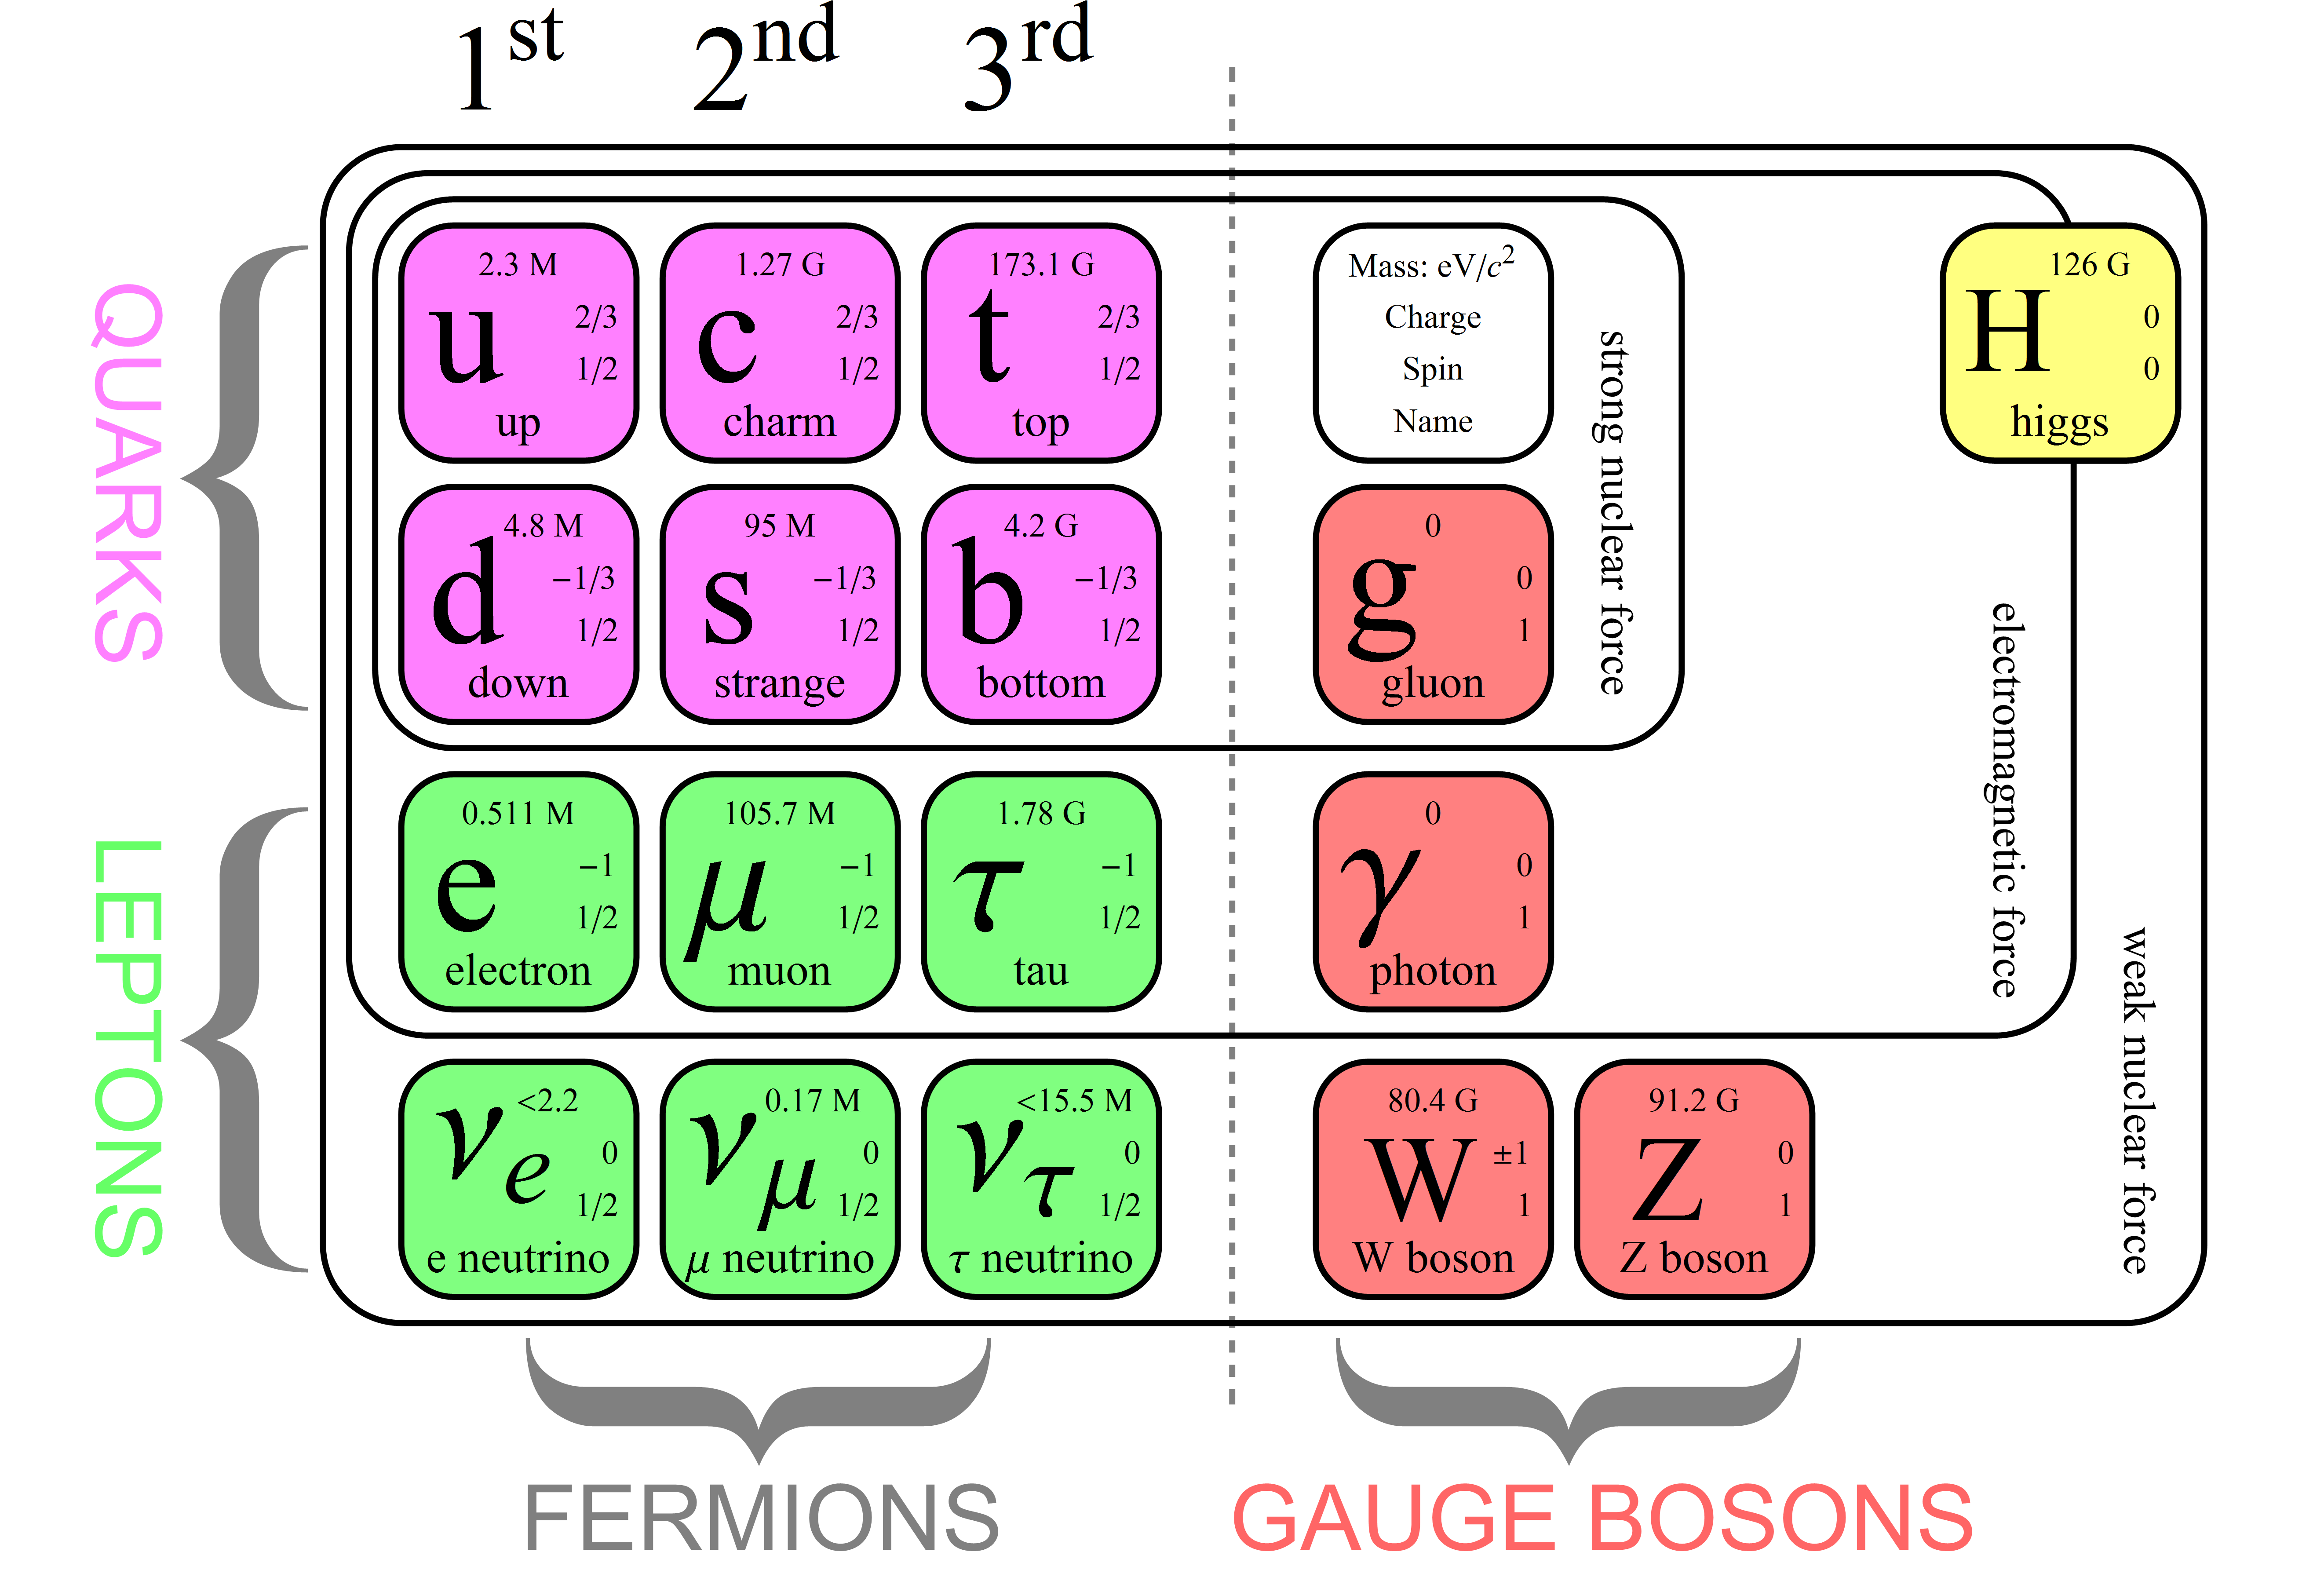
\includegraphics[width=0.98\textwidth]{./plots/SM.png}
  \caption{The particles of the Standard Model.}
  \label{fig:SMParticles}
\end{figure}

\ \\There are 12 fermions representing the constituents of matter. They have a semi-integer spin ($1/2$) and they can be divided into two categories: quarks and leptons. The quarks have fractional electric charges and form barions and mesons. They six quarks are up ($u\,^{+2/3}$), down ($d\,^{-1/3}$), charm ($c\,^{+2/3}$), strange ($s\,^{-1/3}$), top ($t\,^{+2/3}$), and bottom ($b\,^{-1/3}$). The three electrically-charged leptons have a negative charge: the electron ($e\,^{-}$), the muon ($\mu\,^{-}$), and the tau lepton ($\tau\,^{-}$). These have corresponding neutrally-charged leptons caled neutrinos ($\nu_e\,^0$, $\nu_\mu\,^0$, $\nu_\tau\,^0$). These particles form matter. For each matter particle there is an anti-matter particle that has an opposite electric charge. 

\ \\Fermions interact with each other via the echange of other elementary particles called bosons. Bosons are carriers of the elementary forces and have an integer spin ($1$). There are eight type of gluons ($g$) that carry the strong force. The photon ($\gamma$) is responsible for the electromagnetic force. The \Wplus, \Wminus~and the \Zzero~bosons carry the weak force. 

\ \\There is also another type of boson, a scalar elementary particle of spin zero (0), called the Higgs boson. The Higgs boson is the latest elementary particle discovered, in 2012, by the ATLAS and CMS detectors at CERN. It is predicted by the mechanism that explains how the elementary particles acquire mass.

\subsection{The top quark}
\label{sec:TopQuark}

The top quark ($t$) is a very interesting elementary particle to study, for several reasons. It is the heaviest particle from the SM, with a mass \mt=173.3~\GeVcc. This implies the top quark has the highest Yukawa coupling constant. The top quark decays very quickly ($\tau=10^{-25}$ s), before having the time to hadronize, meaning to form stable hadrons. Therefore it is the only quark that can be studied alone. It is observed indirectly through its decay products. The top quark was discovered in 1994 independently by the CDF and DZero experiments at FermiLab in proton-antiproton ($p\bar{p}$) collisions at $\sqrt{s}=1.8$ TeV.

\ \\Measuring the top-quark properties is key to test the validity of the SM. The ATLAS and CMS experiments at CERN measure the properties of the top quark in great detail. If deviations are found in the top quark properties with respect to the SM predictions (\emph{e.g.} different cross-sections), it implies the existence of new physics phenomena beyond the Standard Model (BSM). This would produce a revolution in particle physics, as the SM has not been contradicted by any experiment since its creation in the 1960s. 

\ \\The top quarks are produced in pairs by strong interactions. The Feynman diagrams for the leading order are illustrated in Figure~\ref{fig:TopQuarkFeynmanDiagrams}. At the LHC the quark-antiquark annihilation (left) represents 10\% of the cases, while the gluon-gluon fusion (center and right) represent 90\% of cases. The LHC has a very high luminosity and produces large quantities of top quarks. For this reason the LHC is considered to be also a top-quark factory.

\begin{figure}[h]
  \centering
  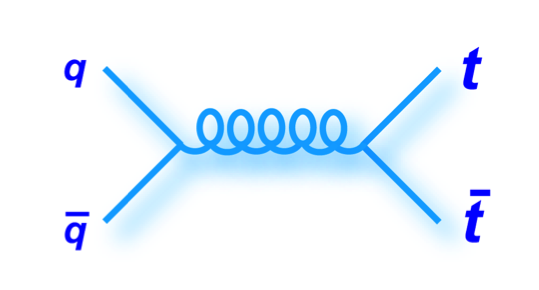
\includegraphics[width=0.32\textwidth]{../presentation/plots/ttbar_1.png}
  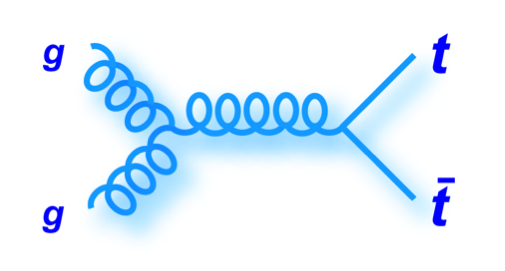
\includegraphics[width=0.32\textwidth]{../presentation/plots/ttbar_2.png}
  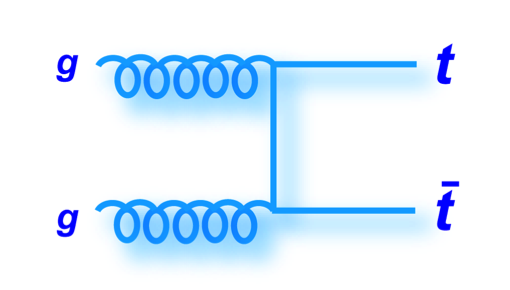
\includegraphics[width=0.32\textwidth]{../presentation/plots/ttbar_3.png}
  \caption{The Feynaman diagrams for the top-quark pair production. At the LHC the quark-antiquark annihilation (left) represents 10\% of the cases, while the gluon-gluon fusion (center and right) represent 90\% of cases.}
  \label{fig:TopQuarkFeynmanDiagrams}
\end{figure}

\ \\The top quark decays in almost 100\% of the time in a \Wboson~and a bottom ($b$) quark. The $W$ boson can decay either to a pair of a quark or an antiquark ($W\rightarrow q\bar{q}$), or to a pair of leptons ($W \rightarrow e\bar{\nu}_e$, $W \rightarrow \mu\bar{\nu}_\mu$, $W \rightarrow \tau\bar{\nu}_\tau$). The $\tau$ lepton decays further leaving as a visible signature in the detector an electron, a muon or two quarks. Since there are two top quarks, they decay to two \Wboson~bosons and two $b$ quarks. Quarks hadronise and appear in the detector as streams of collimated particles called jets. 

\ \\Counting the number of charged leptons (electrons or muons), the top quark events can be grouped into three categories: di-lepton, lepton+jets (one lepton plus jets), and all-hadronic (only jets). The percentage of decay for each case, called branching ratio (BR) is presented in the left-hand side of Figure~\ref{fig:TopQuarkDecay}. In this report we study the subset of the di-lepton with an electron or a muon. The \ttbaremu~decay is present in only 2\% of the cases. It is advantageous because the background is very low comparing to others decay channels. The background comes in most of the cases from the \Zboson~boson decay plus other jets. The full Feynman diagram of production and decay of the \ttbaremu~is presented in the right-hand side of Figure~\ref{fig:TopQuarkDecay}. The latest ATLAS paper on the \ttbaremu~analysis is presented in~\cite{ttbaremu}.

\begin{figure}[h]
  \centering
  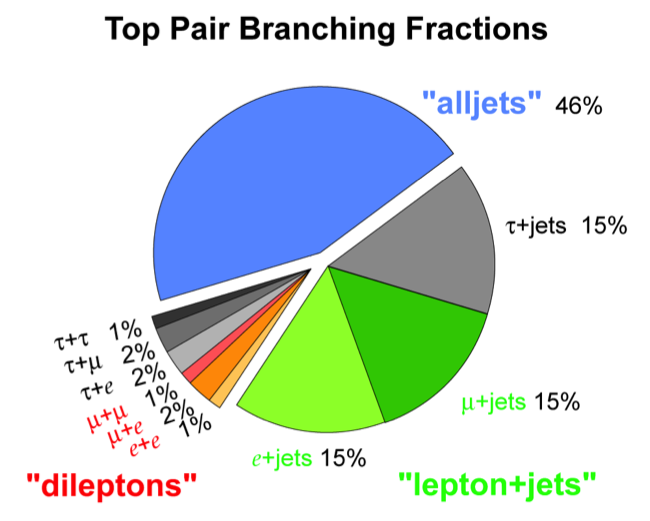
\includegraphics[width=0.47\textwidth]{../presentation/plots/ttbar_5.png}
  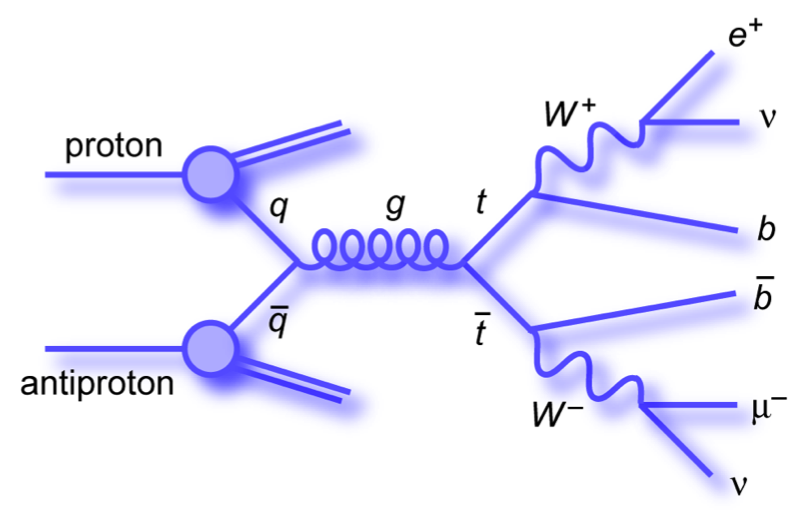
\includegraphics[width=0.47\textwidth]{../presentation/plots/ttbar_4.png}
  \caption{Left: the pie chart of the top-quark pair decay. Right: the Feynman diagram including production and decay of the \ttbaremu~process.}
  \label{fig:TopQuarkDecay}
\end{figure}

\subsection{The experimental setup}
\label{sec:ExperimentalSetup}

The experimental setup used in this study is from the ATLAS experiment at CERN.

\ \\At the moment, the Large Hadron Collider (LHC), which is situated at CERN, is the most powerful proton-proton collider in the world, as illustrated in Figure~\ref{fig:LHC}. After the Tevatron and the Large Electron-Positron Collider (LEP) era, a new machine was needed for new discoveries in particle physics. The LHC was designed to achieve a center-of-mass energy $\sqrt{s}=14\,TeV$. Two of the biggest goals of the LHC are to study the Standard Model and to test its validity.  

\begin{figure}[h]
  \centering
  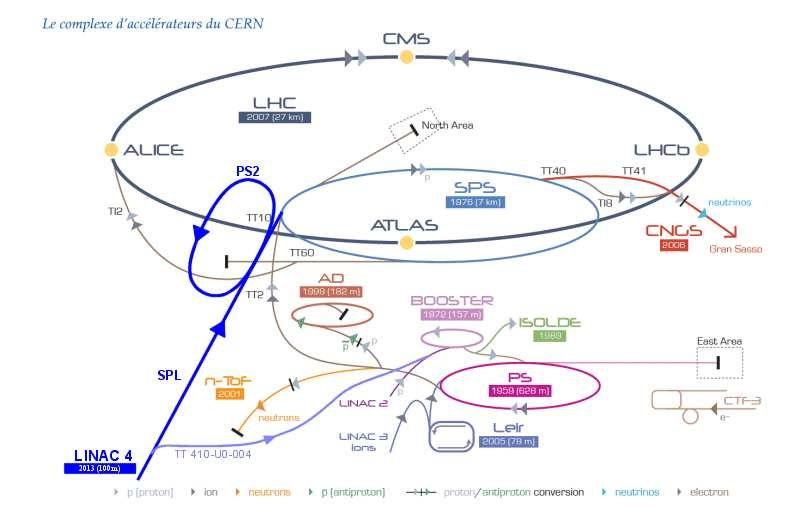
\includegraphics[width=0.5\textwidth]{plots/LHC.png} 
  \caption{The LHC Accelerator Complex System.}
  \label{fig:LHC}
\end{figure}

\ \\This project is affiliated to the international collaboration of the A Toroidal LHC ApparatuS (ATLAS)~\cite{ATLAS}. ATLAS is the largest of the four LHC detectors. ATLAS is one of the two general-purpose particle physics detectors at the LHC, the other being CMS. The two detectors and collaborations perform a similar research program. A new discovery must be observed by both detectors to be believed as true. ATLAS and its subdetectors is illustrated in Figure~\ref{fig:ATLAS}.

\begin{figure}[h]
  \centering
  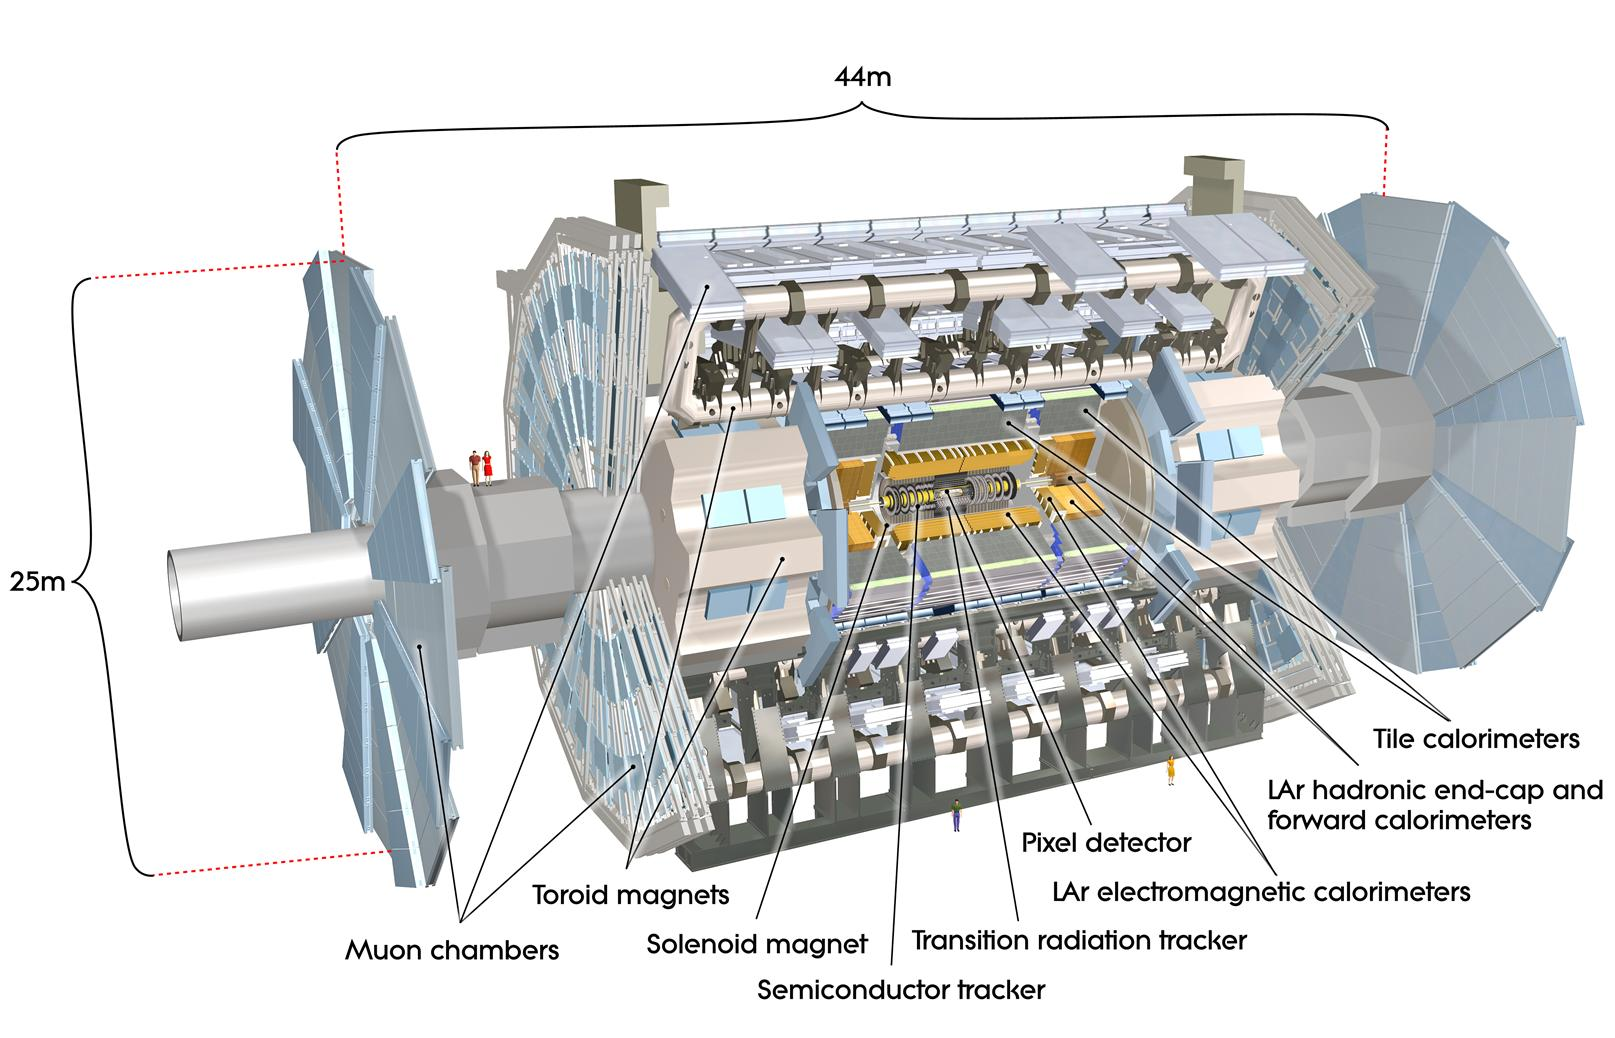
\includegraphics[width=0.5\textwidth]{plots/ATLAS.jpg} 
  \caption{The ATLAS detector and its sub-detectors.}
  \label{fig:ATLAS}
\end{figure}

\ \\ This report presents results obtained using 43076 simulated events of the \ttbaremu~process within the ATLAS experiment~\cite{RootFile}. After an event selection, for each event there is the information available at the reconstructed stage (measured) stage and at the truth (generated) stage. The study focuses on the jet with the highest transverse momentum (\pt), also called the leading jet, in the interval from 0 to 500 \GeV, with a constant bin width of 20 \GeV, which results in 25 bins in total.

\section{Neural Networks}
\label{sec:NeuralNetworks}

\subsection{The method}
\label{sec:Method}

My first step was to study a code example using some toy data in a JupyterNotebook~\cite{AGlazov}. At the beginning I ran the code on a cloud (Swan). 

\ \\The next step was to run it on \texttt{lxplus}. For this it was needed to run after \texttt{ssh}-ing to a \texttt{lxplus} machine a singularity command~\cite{Singularity} and then to my own laptop.

\ \\To train the neural network it was needed to use the Python library Keras~\cite{keras} and for backend TensorFlow~\cite{tensorflow}. My method of sampling was implemented using numpy~\cite{numpy}.

The goal of this project is to adapt a code example of machine learning unfolding (MLUnfolding) using toy data to use it for the jet energy reconstruction of \ttbaremu~analysis.

\ \\In this project one of the problems that we want to solve is the correction of detector smearing using Machine Learning (ML). I have implemented this method using a sequential Neural Network. The unfolding corresponds to an inversion of the migration matrix. Unfolding is the procedure to infer the truth data (what happens in reality in nature) from the reconstructed data (observed and measured in our experiment by our detector). The categorisation is a common problem for the modern Machine Learning methods. Possible methods could be Boosted Decision Trees (BDT) and Artificial Neural Networks (ANN), or in short Neural Networks (NN). NNs with various architectures can be tried for the unfolding problem. The unfolding involves several iterative steps of ML using a NN training in TensorFlow via Keras, in Python. The NN takes as input the reconstructed values, and has as output the truth values.

\ \\The goal of the study is to adapt this example to use real data coming from the jet \pt~distribution from the \ttbaremu~analysis. We use this \texttt{.root} flat tree~\cite{RootFile}. This file contains both the reconstructed and truth jets, already matched. Meaning the i$^{\rm th}$ event from reco, corresponds to the i$^{\rm th}$ event from truth. Each jet collection contains jets already the jets ranked by \pt. We take index 0 to consider the leading reco jet and the leading truth jet.

\ \\Given the leading jet \pt~as a continuous reco value, we want to find out in which jet \pt~bin does the truth jet falls. The jet bin is configurable, say 10 \GeV, or 20 \GeV. The input is a continuous value, but the output is a discrete value, that can take values from 0 to 24 if we consider 20 \GeV~bins from 0 to 500 \GeV. For example, bin index 0 contains jets with \pt~from 0 to 20 \GeV, bin index 1 contains jets with \pt~from 20 \GeV~to 40 \GeV, \emph{etc.}. Jets with \pt~larger than 500 \GeV~have values set by hand to 499.999 \GeV, and enter in the last possible bin index, number 24. It is equivalent to moving the overflow bin of a histogram to the last bin of the histogram. 

\ \\Given the output can take any value from 0 to 24, the problem we try to solve is a classification, and the possible labels are not only two (as in a simple signal to background classification, typically used in ATLAS), but a more complex one, with 25 labels. The NN will return the probability that for a given jet its \pt~falls in any of these bins. The total probability for all bins must be 1.0. This is ensured by the \emph{softmax} activation function for the last layer of the NN. We then consider the bin with the largest probability as our choice by the NN. The predicted bin value can then be compared with the true bin value when making the plots of this project.

\ \\To optimize the NN performance, we take as input in fact not the jet \pt, but the jet \pt~divided by the bin width. This is the jet \pt~bin as a real value. Making things more consistent with the output being the integer jet \pt~bin value for the truth.

\ \\ Neural Networks are an example of Machine Learning. In this way the computers learn a solution for a problem without being explicitly programmed. The two main classes of ML are supervised and unsupervised. 
In this project I used supervised ML. ......~\cite{AndrewNg}.

\ \\If we have the function Pi(y), a multidimensional highly non-linear, an efficient way to do this procedure is with an NN. This was inspired by the brain structure, which contains millions of neurone cells forming a network with electrochemical impulses passing between them. An artificial neural network formed by a number of interconnected artificial \emph{neurons}, or "nodes" respects this architecture. 

\ \\A network is formed by several ayers of nodes connected in series. Each node takes a weighted linear combination of the outputs from nodes of the previous layer, applies "activation function", then outputs the result do the next layer~\cite{AndrewNg}.

\ \\Using a "loss" function we can describe the difference between the predicted and real outputs, like the mean squared error between real and predicted. The weights associated with each node is modifies via an algorithm, and from here we can deduce that the loss function decreases and training increases.

\ \\We know from The \emph{Universal Approximation Theorem} that a neural network with one \emph{hidden layer} of nodes between input and output can in principle approximate any N-dimensional function to an arbitrary degree of accuracy, given a sufficiently large (though finite) number of nodes. 

\ \\In practice it is more suitable to use multiple hidden layers connected in series~\cite{AndrewNg}.

\section{The method}
\label{sec:Method}

My first step was to study a code example using some toy data in a JupyterNotebook~\cite{AGlazov}. At the beginning I ran the code on a cloud (Swan). 

\ \\The next step was to run it on \texttt{lxplus}. For this it was needed to run after \texttt{ssh}-ing to a \texttt{lxplus} machine a singularity command~\cite{Singularity} and then to my own laptop.

\ \\To train the neural network it was needed to use the Python library Keras~\cite{keras} and for backend TensorFlow~\cite{tensorflow}. My method of sampling was implemented using numpy~\cite{numpy}.

\begin{thebibliography}{11}

\bibitem{ATLAS} The ATLAS experiment, \url{https://atlas.cern}
\bibitem{RootFile} The \ttbaremu~ROOT file used {\tiny \texttt{\detokenize{/afs/cern.ch/user/l/lciucu/public/data/MLUnfolding/user.yili.18448069._000001.output.sync.root}}}
\bibitem{bendavid} Joshua Bendavid, \textit{Efficient Monte Carlo Integration Using Boosted Decision Trees and Generative Deep Neural Networks}, 2017
\bibitem{AndrewNg} Andrew Ng, \textit{Machine Learning. Coursera online course}, \url{URL https://www.coursera.org/learn/machine learning}
\bibitem{AGlazov} Alexander Glazov, \textit{Machine learning as an instrument for data unfolding}, \textbf{arXiv}: 1712.01814v1, \url{http://inspirehep.net/record/1641082}
\bibitem{AGlazovCode} Alexander Glazov, \textit{Toy data example for machine learning as an instrument  for data unfolding using TensorFlow via Keras in a Python Jupyter Notebook}, \url{https://github.com/aglazov/MLUnfold/blob/master/Unfold.ipynb}
\bibitem{Singularity} The singularity command to run the ML environment, \\ {\tiny \texttt {\detokenize{singularity exec '/cvmfs/unpacked.cern.ch/registry.hub.docker.com/atlasml/ml-base:latest'bash}}}
\bibitem{keras} The keras machine learning library, \url{https://keras.io}
\bibitem{tensorflow} The TensorFlow machine learning library, \url{https:// www.tensforflow.org}
\bibitem{numpy} The Numerical Python library, \url{https://www.numpy.org}
\bibitem{topquark} \textit{Measurement of jet activity produced in top-quark events with an electron, a muon and two b-tagged jets in the final state in pp collision at s=13 TeV with the ATLAS detector}, \textbf{arXiv}: 1610.09978v2, \url{https://arxiv.org/pdf/1610.09978.pdf}
\bibitem{ReportYichenLi} Yichen Li, \textit{ZUnfold framework, an unfolding framework written at Zeuthen}, \url{http://www.desy.de/~liyichen/Unfolding.pdf}
\bibitem{UnfoldingStatSchool}, Stefan Schmitt, Daniel Brizger, \textit{Slides Unfolding in High Energy Physics at the Terascale statistics school 2014}, \url{http://www.desy.de/~sschmitt/talks/UnfoldStatSchool2014.pdf?fbclid=IwAR3CB3CwJOQchKfbZRIg6ktRf6DbI5KTD5cdtBbNHS1lKb-q3yrwagyua5w}.

\end{thebibliography}


\end{document}








\end{thebibliography}

\end{document}

%%%%%%%%%%%%%%%%%%%%%%%%%%%%%%%%%%%%%%%%%%
%%% example code - do not write below
%%%%%%%%%%%%%%%%%%%%%%%%%%%%%%%%%%%%%%%%%%%

\section{Introduction}

\subsection{Part 1...}

\paragraph{}
Here new paragraph starts...........
\paragraph{}
Here new paragraph starts...........
\paragraph{}
Here new paragraph starts........... \\

\newpage
		
Equation:
	
\begin{equation}
% \langle t_f q_f | t_i q_i \rangle = 
\lim_{\substack{\epsilon \rightarrow
0\\N\rightarrow \infty}} \int \dots \int \mbox{d}q_1 \dots \mbox{d}q_{N-1} \frac{\mbox{d}p_1}{2 \pi
\hbar} \dots \frac{\mbox{d}p_N}{2 \pi \hbar}\exp{\left( \frac{i}{\hbar} \sum_{j=1}^N
\left[ p_j (q_j - q_{j-1}) - \epsilon H\left(pj, \frac{q_j +
q_{j-1}}{2}\right)\right]\right)}
\end{equation}
\vspace{2cm}
\begin{align}
 \lim_{\substack{\epsilon \rightarrow 0 \\ N\rightarrow \infty}} \frac{i}{\hbar}
\epsilon \sum_{j=1}^N \left[p_j \left(\frac{q_j-q_{j-1}}{\epsilon}\right) - H\left( p_j,
\frac{q_j+q_{j-1}}{2}\right) \right] &= \frac{i}{\hbar} \int_{t_i}^{t_f} \mbox{d}t \left( p
\dot{q}-H(p,q)\right) \nonumber\\ 
&= \frac{i}{\hbar} \int_{t_i}^{t_f} \mbox{d}t L = \frac{i}{\hbar} S[q]
\end{align}
\vspace{2cm}

Table:

Consider the following mesons $\eta$, $\eta'$ and $K$ and their quark content\footnote{The mesons
are actually a superposition of these quarks.}:
\begin{center}
\begin{tabular}{c|c|c}
 meson & composition & approx. mass\\ \hline
$K^0$ &  $d\bar{s} \, , \,s\bar{d}$ &  $498 \mbox{MeV}$\\
$K^{+}$ & $u\bar{s}$ & $494 \mbox{MeV}$\\
$K^{-}$ & $s \bar{u}$ & $494 \mbox{MeV}$  \\
$\eta$ & $u \bar{u} \, , \, d \bar{d} \, , \, s \bar{s}$ & $548 \mbox{MeV}$ \\
$\eta'$ & $u \bar{u} \, , \, d \bar{d} \, , \, s \bar{s}$ & $958 \mbox{MeV}$ 
\end{tabular}
\end{center}


\newpage
	
Plot:

\begin{figure}[h]
\subfloat{\includegraphics[width=0.495\textwidth]{figure.jpg}}%\label{corr_and_rate-left}}
\subfloat{\includegraphics[width=0.495\textwidth]{figure.jpg}}%\label{corr_and_rate-right}}
\caption{Left: correlation for different $d$ ; Right: acceptance rate and
autocorrelation time for different $d$}
\label{corr_and_rate}
\end{figure}

\newpage
		
\subsection{Part 2...}

\paragraph{}
Here new paragraph starts...............................................................
...........................................................................................
..........................................................................................
...........................................................................................
\paragraph{}
Here new paragraph starts..........................................................................
...........................................................................................
..........................................................................................
...........................................................................................
\paragraph{}
Here new paragraph starts..........................................................................
...........................................................................................
..........................................................................................
........................................................................................... \\

\section{Conclusions}

Some text here..............................................................................

\section*{Acknowledgements}

Some text here..............................................................................

\begin{thebibliography}{11}
\bibitem{nagashima}
Yorikiyo Nagashima, Yoichiro Nambu, \textit{Elementary Particle Physics Volume 1: Quantum Field
Theory and Particles}, (WILEY-VCH, 2010)
\bibitem{FORTRAN}
W. H. Press, S. A. Teukolsky, W. T. Vetterling, B. P. Flannery, \textit{Numerical Recipes in
FORTRAN - The Art of Scientific Computing, 2nd Ed.} (Cambridge University Press, 1992)
\bibitem{buendia}
G. M. Buend\'{i}a, \textit{Comparison between the Langevin and the hybrid simulation techniques for
a free field theory}, J. Phys. A: Math. Gen. \textbf{22}, 5065-5072 (1989).
\bibitem{tapei}
T. Cheung and L. Li, \textit{Gauge theory of elementary particle physics}, (Oxford University
Press, 1984)
\bibitem{degrand}
T. DeGrand and C. DeTar, \textit{Lattice Methods for Quantum Chromodynamics}, (World Scientific,
2006)
\bibitem{topoactions}
W. Bietenholz, U. Gerber, M. Pepe, U.-J. Wiese, \textit{Topological Lattice Actions},
arXiv:1009.2146v4 [hep-lat] (20 Dec 2010)
\bibitem{openbcs}
M. L\"{u}scher, S. Schaefer, \textit{Lattice QCD without topology barriers},
CERN-PH-TH-2011-116, 26pp (May 2011)
\bibitem{Crecipes}
W. H. Press, S. A. Teukolsky, W. T. Vetterling, B. P. Flannery, \textit{Numerical Recipes in
C - The Art of Scientific Computing, 2nd Ed.} (Cambridge University Press, 1992)
\bibitem{andreas}
A. Nube, private communication.
\bibitem{wolff}
U. Wolff, \textit{Critical Slowing Down}, Nuclear Physics B (Proc. Suppl.) \textbf{17}, 93-102
(1990).
\end{thebibliography}
\end{document}
